% Two subfloats so the text can reference each panel on its own
% (\autoref{fig:rq1_method} and \autoref{fig:rq1_best_spectral}), or the pair
% as \autoref{fig:rq1_score_distributions}.
%
% Both PDFs are built by research/rq1/export_figure_pdfs.py into figures/.
% They are drawn to be read as one stacked figure: the top panel carries the
% legend and no x-axis numbers, the bottom panel carries the x-axis and no
% legend. Keep them in this order and at the same width.
\begin{figure}[!htbp]
    \centering

    \subfloat[\method{} Sepctrum + No Train.]{
        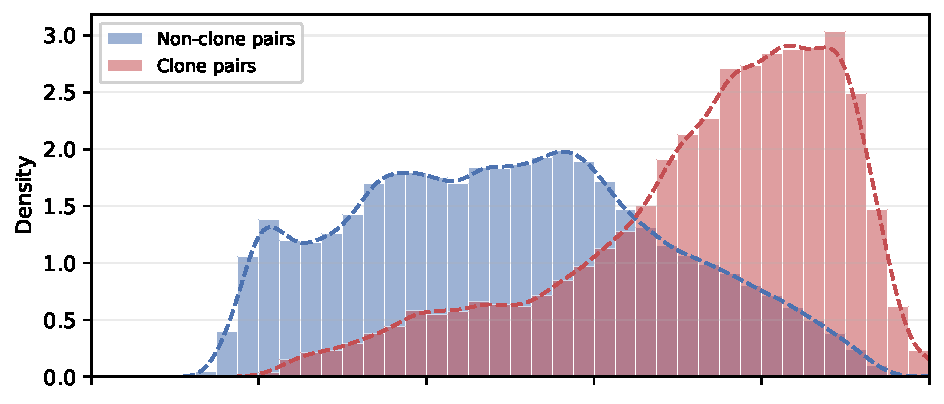
\includegraphics[
            width=0.98\columnwidth,
            height=0.15\textheight
        ]{figures/latent_NoTrain.pdf}
        \label{fig:rq1_method}
    }

    \vspace{2mm}

    \subfloat[AST + No Train.]{
        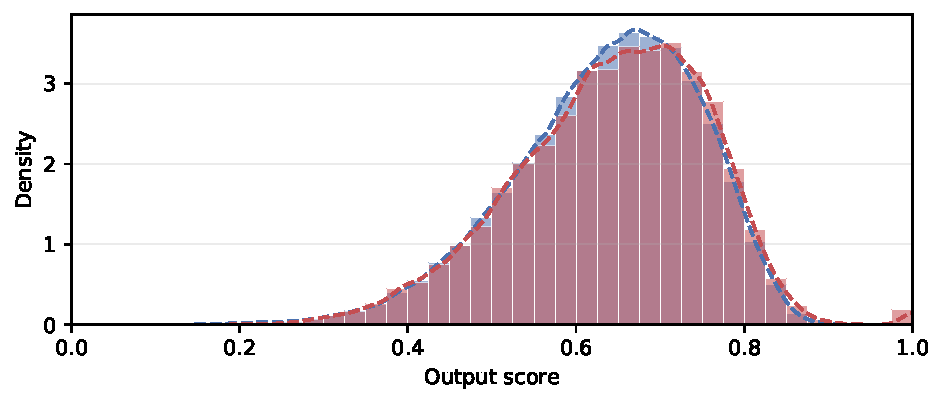
\includegraphics[
            width=0.98\columnwidth,
            height=0.15\textheight
        ]{figures/ast_NoTrain.pdf}
        \label{fig:rq1_best_spectral}
    }

    \caption{Output-score distributions on BigCloneBench for the learned latent spectrum of \method{} and the fixed AST spectrum, both evaluated without a learned downstream prediction head.}
    \label{fig:rq1_score_distributions}
\end{figure}
